\week{October 2, 1993}

I think I'll depart from my usual concerns this week and talk about a book I'd been meaning to get my hands on for ages:

\find{\paper{John H. Conway and Neil J. A. Sloane, Sphere Packings, Lattices and Groups, second edition, Grundlehren der mathematischen Wissenschaften 290, Springer-Verlag, 1993.}}

This is a mind-boggling book. I have always regarded research in combinatorics as a pleasure I must deny myself, for the study of the \emph{discrete} presents endless beautiful tapestries in which one could easily lose oneself for life, and I regard this as a kind of self-indulgence when there is, after all, the physical universe out there waiting to be understood. Of course, it's good that \emph{someone} does combinatorics, since even the most obscure corners have a strong tendency to become useful eventually - and if they write books about it, I can have my cake and eat it too, by \emph{reading} about it. Conway and Sloane are two masters of combinatorics, and this book is like a dessert tray piled so high with delicacies that it's hard to know where to begin. Rather than attempt to describe it, let me simply show you a few things I found in it. The book is 679 pages long, so what I'll say is only the most minute sample!

Let's begin with sphere packings. Say one is stacking cannonballs on ones lawn, which is a quaint custom now that cannons have been replaced by far more horrible weapons. A nice way to do it is to lay out a triangle of cannonballs thus:
\begin{center}
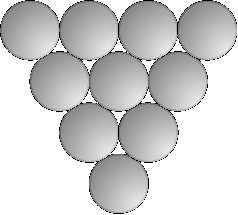
\includegraphics[]{figures/wk20_fig1.pdf}
\end{center}
and then set down another triangle of cannonballs on top of the first layer, one in every other hole, thus:
\begin{center}
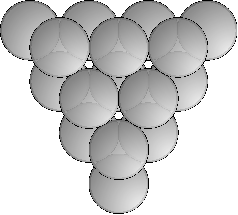
\includegraphics[]{figures/wk20_fig2.pdf}
\end{center}

and another:
\begin{center}
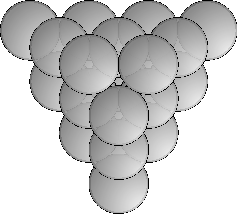
\includegraphics[]{figures/wk20_fig3.pdf}
\end{center}

and finally one on top - which I won't attempt to draw. Very nice stack! There are many mathematical reflections it could lead one to, one of which is: is this the \emph{densest} possible way one can pack spheres of equal radius? The density is $\frac{\pi}{\sqrt{18}} = .7405...$; can one do better? Apparently it was Kepler who first conjectured that the answer is ``no.'' This is a famous hard problem. In 1991 W.-Y. Hsiang announced that he had a proof, but I am not sure how many experts have read it and been convinced.

This packing is a very regular sort of packing, what people call a lattice packing. A lattice is a discrete subset of $n$-dimensional Euclidean space closed under addition, and the packing above corresponds to a lattice called the ``face-centered cubic'' or fcc lattice, which is the set of all points $(x,y,z)$ where $x, y,\text{ and }z$ are integers adding up to an \emph{even} number. (One might have a bit of fun drawing some of those points and seeing why they do the job.) Naturally, because of their regularity lattice packings are easier to study than non-lattice ones. In fact, Gauss showed in 1831 that the fcc lattice is the densest of all \emph{lattice} packings of spheres in 3 dimensions. This justifies the practice of stacking grapefruit this way in the supermarket.

Let's take a bit closer look at what's going on here. Imagine an fcc lattice going off infinitely in all directions... each sphere is touching 12 others: 6 in its own layer, as it were, 3 in the layer above and 3 in the layer below. If we only pay attention to a given sphere and those touching it we see something like:
\begin{center}
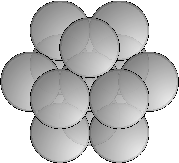
\includegraphics[]{figures/wk20_fig4.pdf}
\end{center}
If we remove the central sphere to clean up the picture a bit, the centers of the remaining are the vertices of a shape called the cuboctahedron:
\begin{center}
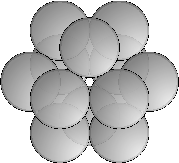
\includegraphics[]{figures/wk20_fig5.pdf}
\end{center}
It has 12 vertices, 8 triangular faces, and 6 square faces. One can get it either by cutting off the corners of a cube just right, or by cutting off the corners of an octahedron!

Let's return to thinking about the 12 spheres touching the central one. This raises another question: is 12 the largest number of equal-radius spheres able to touch a given one? This is the ``kissing spheres'' problem - not quite the same as the packing problem! In 1694, Newton conjectured that 12 was the largest number one could achieve. His correspondent, David Gregory, thought 13 might be possible. It turns out that Newton was right (some proofs appeared in the late 1800's), but it is important to realize that Gregory's guess was not as dumb as it might sound!

Why? Well, there's another way to get 12 spheres to touch a central one. Namely, locate them at the vertices of a (regular) icosahedron. If one wants to get to know the icosahedron a bit better one might read my article \href{http://math.ucr.edu/home/baez/six.html}{Some Thoughts on the Number Six}. But I hope you have an icosahedron available, or at least a good mental image of one. It's easy to describe the vertices of the icosahedron mathematically in terms of the golden ratio,

\[ \frac{\sqrt{5} + 1}{2} = 1.61803398874989484820458683437....\]
This usually goes by the name of ``$\phi$,'' or sometimes ``$\tau$,'' but for brevity I'll use ``$G$'' for this number. The magic properties of $G$ are too numerous to list here, but what counts is that one gets the 12 vertices of a (regular) icosahedron by taking the points

\[                (\pm G, \pm 1, 0),\]
\[                (\pm 1, 0, \pm G),\]
\[                (0, \pm G, \pm 1).\]
This is easy to check.

Now the \emph{interesting} thing is that when one gets 12 spheres to touch a central one using the icosahedron, the 12 sphere don't touch each other! There's room to move 'em around a bit, and perhaps (thought Gregory) even enough room to stick in another one! Well, Gregory was wrong, but one can do something pretty cool with this wiggle room. First, though, let's check that there really \emph{is} a little space between those outer spheres. First, compute the distance between neighboring vertices of the icosahedron by taking two and working it out:

\[               ||(G,1,0) - (G,-1,0)|| = 2.\]
Then, compute the distance from any of the vertices to the origin, which is the center of the central sphere:

\[               ||(G,1,0)|| = \sqrt{G^2 + 1}.\]
Using the charming fact that $G^2 = G + 1$ this simplifies to $\sqrt{G + 2}$, but then I guess we just need to grind it out:

\[ \sqrt{G + 2} =  1.902....\]
The point is that this is less than 2, so two neighboring spheres surrounding the central one are farther from each other than from the central one, i.e., they don't touch.

Now here's an interesting question: say we labelled the 12 spheres touching the central one with numbers 1--12. Is there enough room to roll these spheres around, always touching the central one, and permute the spheres 1--12 in an interesting way? Notice that it's trivially easy to roll them around in a way that amounts to rotating the icosahedron, but are there more interesting permutations one can get?

Recall that the group of permutations of 12 things is called $S_{12}$, and it has

\[ 12! = 479001600\]
elements. The rotational symmetry group of the icosahedron is much smaller. One can count its elements as follows: pick a vertex and say which new vertex it gets rotated to - there are 12 possibilities - and then note that there are 5 ways that could have happened, for a total of 60. In fact (as I show in the article \href{http://math.ucr.edu/home/baez/six.html}{``Six''}) the rotational symmetry group of the icosahedron is $A_5$, the group of \emph{even} permutations of 5 things. So we have a nice embedding of the group $A_5$ into $S_{12}$, but we are hoping that by some clever wiggling we can get a bigger subgroup of $S_{12}$ as the group of permutations we can achieve by rolling spheres around.

In fact, one can achieve all EVEN permutations of the 12 spheres this way! In other words, we get the group $A_{12}$, with

\[ \frac{12!}{2} = 239500800\]
elements. How? Well, I wish I could draw an icosahedron for you, but I can't really do so well on this medium. The best way is to draw a top view:
\begin{center}
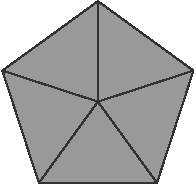
\includegraphics[]{figures/wk20_fig6.pdf}
\end{center}
and a bottom view:
\begin{center}
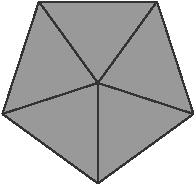
\includegraphics[]{figures/wk20_fig7.pdf}
\end{center}
Now, if we take the top 6 spheres and bunch them up so they are all touching, and the bottom 6 spheres and bunch them up so they all touch, we can, in fact, twist the top 6 counterclockwise around 1/5 of a turn. That is, we can map
\begin{center}
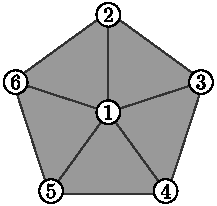
\includegraphics[]{figures/wk20_fig8.pdf}
\end{center}
to
\begin{center}
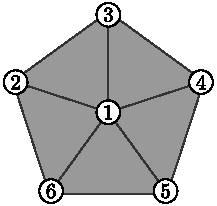
\includegraphics[]{figures/wk20_fig9.pdf}
\end{center}

I haven't actually \emph{done} this, or even proved I can, but Conway and Sloane say so. And then the point is that all of $A_{12}$ is generated by ``twists'' of this form. Conway and Sloane give a sophisticated and quick proof of this fact, which I can't resist mentioning. Readers who don't know much group theory can skip the next paragraph!

First, let $t(i)$ be the element of $S_{12}$ corresponding to the clockwise twist about the $i$th vertex of the icosahedron (so that what's drawn above is $t(1))$. This is a 5-cycle, and we need to show these 12 5-cycles generate $A_{12}$. Consider the subgroup generated by elements of the form $t(i)t(j)^{-1}$ -- a clockwise twist followed by a counterclockwise twist. This is the Mathieu group $M_{12}$, a most remarkable group! In particular, its action on the vertices of the icosahedron is able to map any 5 vertices to any 5 others (we say it's quintuply transitive), so by conjugating $t(i)$ with elements of the Mathieu group we can get any 5-cycle in $S_{12}$. Then we use the fact that $A_{12}$ is generated by the 5-cycles.

Anyway, what this indicates is that there is an interesting relation between the icosahedron and a certain finite group, the Mathieu group $M_{12}$. This group has

\[ \frac{12!}{7!} = 95040 \]
elements and it is a ``simple'' group, in the technical sense. The simple groups are to finite groups roughly as the prime numbers are to the counting numbers; that is, they are the elementary building blocks from which other finite groups are made (although one has to specify \emph{how} one gloms them together to get other groups). One of the remarkable achievements of this century is the classification of these simple groups. In addition to various infinite families of simple groups, like the alternating groups An (consisting of even permutations) there are a finite number of ``sporadic'' simple groups such as the Mathieu groups, the Fischer groups, the Suzuki groups, and, biggest of all, the Monster group, which has

\begin{align*} 2^{46} \cdot 3^{20} \cdot 5^9 \cdot 7^6 & \cdot 11^2 \cdot 13^3 \cdot 17 \cdot 19 \cdot 23 \cdot 29 \cdot 31 \cdot 41 \cdot 47 \cdot 59 \cdot 71 = \\
& 808017424794512875886459904961710757005754368000000000 \end{align*}
elements!

Here's a fun story about this number.

In the 1970s, the mathematicians Fricke, Ogg and Thompson were studying the quotient of the hyperbolic plane by various subgroups of SL(2,$\R$) -- the group of $2 \times 2$ real matrices with determinant one -- which acts as isometries of the hyperbolic plane. Sitting inside SL(2,$\R$) is the group of $2 \times 2$ integer matrices with determinant one, called SL(2,$\Z$). Sitting inside that is the group $\Gamma_0(p)$ consisting of matrices whose lower left corner is congruent to zero mod $p$ for the prime $p$. But Fricke, Ogg and Thompson were actually considering a somewhat larger group $\Gamma_0(p)+$, which is the normalizer of $\Gamma_0(p)$ inside SL(2,$\R$).

If you don't know what this stuff means, don't worry! The point is that they asked this question: if we take the quotient of the hyperbolic plane by this group $\Gamma_0(p)+$, when does the resulting Riemann surface have genus zero? And the \emph{real} point is that they found the answer was: precisely when $p$ is 2, 3, 5, 7, 11, 13, 17, 19, 23, 29, 31, 41, 47, 59 or 71.

Later, Ogg went to a talk on the Monster and noticed that these primes were precisely the prime factors of the size of the Monster! He wrote a paper offering a bottle of Jack Daniels whiskey to anyone who could explain this fact. This was the beginning of a subject which Conway dubbed ``Monstrous Moonshine'': the mysterious relation between the Monster group, the group SL(2,$\R$), and Riemann surfaces.

It turns out that lying behind Monstrous Moonshine is a certain string theory having the Monster as symmetries, and this was the key to understanding many strange ``coincidences''.

So, the sporadic groups are telling us something very deep and mysterious about the universe, since they are very complicated and yet somehow a basic, intrinsic part of the weave of mathematics. Conway and Sloane have a lot to say about them and their relations to lattices and error-correcting codes. For more about Monstrous Moonshine and string theory, the reader should try this:

\find{\paper{Igor Frenkel, James Lepowsky, and Arne Meurman, Vertex Operator Algebras and the Monster, Academic Press, New York, 1988.}}

Rather than attempt to describe this work, which I am not really qualified to do (not that that usually stops me!), I think I will finish up by describing a charming connection between the beloved icosahedron and a lattice in 8 dimensions that goes by the name of $E_8$. I'll be a bit more technical here.

The group of rotational symmetries of the icosahedron is, as we have said, $A_5$. This is a subgroup of the 3d rotation group SO(3). As all physicists know, whether they know it or not, the group SO(3) has the group SU(2) of $2 \times 2$ unitary matrices with determinant 1 as its double cover. So we can find a corresponding double cover of $A_5$ as a subgroup of SU(2); this has twice as many elements as $A_5$, for a total of 120.

Now the group SU(2) has a nice description as the group of unit quaternions, that is, things of the form

\[          a + bI + cJ + dK,\]
where $a,b,c,d$ are real numbers with $a^2 + b^2 + c^2 + d^2 = 1$, and $I,J,\text{ and }K$ satisfy
\[IJ = -JI = K, \quad	JK = -KJ = I, \quad   KI = -IK = J, \quad  I^2 = J^2 = K^2 = -1\]
(Physicists in the 20th century usually use the Pauli matrices instead, which are basically the same thing; for the relationship, read ``week5''.)

It's natural to ask what the double cover of $A_5$ looks like explicitly in terms of the unit quaternions. Conway and Sloane give a nice description. Let's write $(a,b,c,d)$ for $a + bI + cJ + dK$, write $G$ for the golden ratio as before, and $g$ for the inverse of the golden ratio:

\[ g = G^{-1} = G - 1 = 0.61803398874989484820458683437....\]
Then the elements of the double cover of $A_5$ are of the form
\[
\begin{array}{lccr}
(\pm 1, & 0, & 0, & 0),\\[1ex]
(\pm \frac{1}{2}, & \pm \frac{1}{2}, & \pm \frac{1}{2}, & \pm \frac{1}{2}),\\[1ex]
(    0, & \pm \frac{1}{2}, & \pm \frac{g}{2}, & \pm \frac{G}{2}),
\end{array}
\]
and everything else that can be gotten by \emph{even} permutations of the coordinates. (Check that there are 120 and that they are closed under multiplication!)
Charming, but what does it have to do with $E_8$? Well, note that if we take all finite sums of elements of the double cover of $A_5$ we get a subring of the quaternions that Conway and Sloane calls the ``icosians.'' Any icosian is of the form

\[           a + bI + cJ + dK,\]
where $a,b,c,\text{ and }d$ live in the ``golden field'' $\Q(G)$ --- this is the field of numbers of the form

\[            x + \sqrt{5} y\]
where $x$ and $y$ are rational. Thus we can think of an icosian as an 8-tuple of rational numbers. We don't get all 8-tuples, however, but only those lying in a given lattice.

In fact, we can put a norm on the icosians as follows. First of all, there is usual quaternionic norm

\[          ||a + bI + cJ + dK||^2 = a^2 + b^2 + c^2 + d^2. \]
But for an icosian this is always of the form $x + \sqrt{5} y$ for some rational $x$ and $y$. It turns out we can define a new norm on the icosians by setting

\[          |a + bI + cJ + dK|^2 = x + y.\]
With respect to this norm, the icosians form a lattice that fits isometrically in 8-dimensional Euclidean space and is the famous one called $E_8$! $E_8$ is known to yield the densest lattice packing of spheres in 8 dimensions, a fact that is not only useful for 8-dimensional greengrocers, but also is apparently used in error-correcting codes in a number of commercially available modems! (If anyone knows \emph{which} modems use $E_8$, let me know - I might just buy one!) The density with which one can pack spheres in 8 dimensions using $E_8$, by the way, is $\frac{\pi^4}{384}$, or about .2537.

Group theorists and some physicists, of course, will know that $E_8$ is also the root lattice of the largest exceptional Lie group, also known as $E_8$. This appears as the gauge group in some string theories. While I find those string theories a bit baroque for my taste, there is clearly a lot of marvelous mathematics floating around here, and anyone who wants more might start with Conway and Sloane.

\Addendum

I had written:
\begin{quote}
Now here's an interesting question: say we labelled the 12 spheres touching the central one with numbers 1--12. Is there enough room to roll these spheres around, always touching the central one, and permute the spheres 1--12 in an interesting way? Notice that it's trivially easy to roll them around in a way that amounts to rotating the icosahedron, but are there more interesting permutations one can get?
In fact, one can achieve all EVEN permutations of the 12 spheres this way!
\end{quote}
I got some email from Conway saying that in fact one get ALL permutations of the 12 spheres. The point is this. One can start with the 12 spheres touching the central one arranged so their centers are at the vertics of an icosahedron. Then one can roll them around so their centers lie at the vertices of a cuboctahedron:
\begin{center}
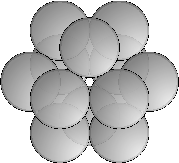
\includegraphics[]{figures/wk20_fig5.pdf}
\end{center}
%\begin{verbatim}
%                         x       x   
%
%                         *   o   * 
% 
%                     x               x
%
%                         o   *   o
%
%                         x       x
%\end{verbatim}
At this point they touch each other, but one can indeed get to this position. There is a nice picture of \emph{how} to do this in Conway and Sloane's book, but you might enjoy figuring it out.
Now if we rotate the cuboctahedron around the axis pointing towards the reader, we get an odd permutation of the 12 spheres, with cycle structure (1 2 3)(4 5 6)(7 8 9 10 11 12). So one can in fact get all of $S_{12}$ if one lets the 12 spheres ``just touch.'' If one thinks about it a bit, the method described in the previous post gets all of $A_{12}$ without the 12 spheres touching at all. Conway says he doesn't know if one can get all of $S_{12}$ without the 12 spheres touching each other at all. So this might be a fun problem to work on. I bet the answer is ``no''.

Conway says the permutation problem came up before a lecture he gave at U. of Penn. a while ago, that he solved it during the lecture, and told Jim Propp about it afterwards.

Someone with much better intuition about these things than I have might want to consider similar ``rolling spheres permutation problems'' in higher dimensions. E.g., what permutations can one can achieve in 4 dimensions, where it is possible to get 24 spheres to touch a central one? (In 4d it is not known whether one can get 25 to touch, but 25 is an upper bound.) Greg Kuperberg informs me that the known method for having 24 spheres touch the central sphere is rigid, so that only the ``obvious'' permutations are possible starting from this arrangement.

The only other cases where the rolling spheres permutation problem appears to be solved is in dimensions 1 and 2 (boring), 8, and 24. I described the $E_8$ lattice in 8 dimensions in ``This Week's Finds.'' In the corresponding lattice packing, each sphere touches 240 others. This is, up to rotation, the \emph{only} way to get 240 spheres to touch a central one in 8 dimensions. (Also, one cannot get \emph{more} than 240 to touch the central one.) So the subgroup of $S_{240}$ that one can get by rolling 240 spheres around a central one is precisely the ``obvious'' subgroup, that is, the subgroup of SO(8) that preserves the $E_8$ lattice. This turns out to be just the Weyl group of $E_8$, which has
\[2^{14} \cdot 3^5 \cdot 5^2 \cdot 7 = 696729600\]
elements.

Dimension 24 is probably the most interesting for lattice theory, and here the densest lattice packing is the Leech lattice. I am somewhat sorry not to have even mentioned the Leech lattice in my article, since this is the real star of Conway and Sloan's book. The Leech lattice is probably related to the appearance of 26-dimensional spacetime in string theory; to get it, start with the unique even unimodular lattice in 26-dimensional Minkowski space, and then look at $M$, the set of vectors in the lattice perpendicular to the vector $w = (70,1,2,3,\dotsc,24)$. This is a null vector since

\[1^2 + 2^2 + \dotsb + 24^2 = 70^2,\]
%
i.e., it is perpendicular to itself. Taking the quotient of $M$ by by $w$ itself, we get the Leech lattice. In this lattice each sphere touches 196560 others, which is the most one can attain, and again this is the only way to get 196560 spheres to touch a central one in 24 dimensions. This should be obvious by visualizing it. :-) So again the answer to the rolling spheres permutation problem is the subgroup of SO(24) that preserves the Leech lattice. The isomorphism group of the Leech lattice is an interesting group called Co${}_0$ or .0 (pronounced ``dotto''). It has

\[2^{22} \cdot 3^9 \cdot 5^4 \cdot 7^2 \cdot 11 \cdot 13 \cdot 23 = 8315553613086720000\]
%
elements. The Monster group can also be produced using the Leech lattice.

Please don't be fooled into thinking I understand this stuff!

Jim Buddenhagen raised another interesting point:
\\
Since 13 unit spheres can't quite all touch a unit sphere, one may ask how much bigger the central sphere must be to allow all 13 to touch.

In 1951 K.\ Schutte and B.L.\ van der Waerden found an arrangement of the 13 unit spheres that allows all of them to touch a central sphere of radius $r=1.04557...$ This is thought to be optimal but has not been proved optimal.

This $r$ is an algebraic number and is a root of the polynomial
%
\[4096 x^{16} - 18432 x^{12} + 24576 x^{10} - 13952 x^8 + 4096 x^6 - 608 x^4 + 32 x^2 + 1.\]
%
They computed $r$ but did not publish the polynomial.
